\documentclass[twoside]{book}

\usepackage[paperwidth=148mm, paperheight=210mm]{geometry}
\usepackage{fontspec}
%\usepackage[latin1]{inputenc}
\usepackage[nolocalmarks]{polyglossia}
\setdefaultlanguage[variant=french, frenchitemlabels=false]{french}
\usepackage[strict]{changepage}
\usepackage{fancyhdr}
\usepackage{paracol}
\usepackage{tableof}
\usepackage{setspace}
\usepackage{alltt}
\usepackage{titlesec}
\usepackage{xcolor}
\usepackage{xstring}
\usepackage{enumitem}

%%%%%%%%%%%%%%%%%%%%%%%%%%%%%%%%%%%%%%%%%%%%%%%%%%% Mise ne page %%%%%%%%%%%%%%%%%%%%%%%%%%%%%%
% on numérote les nbp par page et non globalement
\usepackage[perpage]{footmisc}

% définition des en-têtes et pieds de page
\pagestyle{empty}
\fancyhead{}
\fancyfoot{}
\renewcommand{\headrulewidth}{0pt}
\setlength{\headheight}{10pt}
\fancyhead[RO]{\small\thepage}
\fancyhead[LE]{\small\thepage}
% la commande titres permet de changer les titres de gauche et de droite.
\newcommand{\titres}[2]{
	\renewcommand{\rightmark}{\textcolor{red}{\sc #2}}
	\renewcommand{\leftmark}{\textcolor{red}{\sc #1}}
}
\titres{}{}

% pas d'indentation
\setlength{\parindent}{0mm}

\geometry{
inner=25mm,
outer=12mm,
top=15mm,
bottom=15mm,
headsep=3mm,
}

%%%%%%%%%%%%%%%%%%%%%%%%%%%%%%%%%%%%%%%%%%%%%%%%% Options gregorio %%%%%%%%%%%%%%%%%%%%%%%%%

\usepackage[forcecompile]{gregoriotex}
%\usepackage{gregoriotex}

%% style général de gregorio :
% lignes rouges, commenter pour du noir
%\gresetlinecolor{gregoriocolor}

% texte <alt> (au-dessus de la portée) en rouge et en petit, avec réglage de sa position verticale
\grechangestyle{abovelinestext}{\color{gregoriocolor}\footnotesize}
\newcommand{\altraise}{0 mm}
\grechangedim{abovelinestextraise}{\altraise}{scalable}

% taille des initiales
\newcommand{\initialsize}[1]{
    \grechangestyle{initial}{\fontspec{Zallman Caps}\fontsize{#1}{#1}\selectfont}
}
\newcommand{\defaultinitialsize}{28}
\initialsize{\defaultinitialsize}
% espace avant et après les initiales
\newcommand{\initialspace}[1]{
  \grechangedim{afterinitialshift}{#1}{scalable}
  \grechangedim{beforeinitialshift}{#1}{scalable}
}
\newcommand{\defaultinitialspace}{0cm}
\initialspace{\defaultinitialspace}

%% sélection de la police de neumes
\gresetnabcfont{gresgmodern}{12} 

% on définit le système qui capture des headers pour générer des annotations
% cette commande sera appelée pour définir des abréviations ou autres substitutions
\newcommand{\resultat}{}
\newcommand{\abbrev}[3]{
  \IfSubStr{#1}{#2}{ \renewcommand{\resultat}{#3} }{}
}
\newcommand{\officepartannotation}[1]{
  \renewcommand{\resultat}{#1}
  \abbrev{#1}{ntro}{ {Intr.} }
  \abbrev{#1}{espo}{Resp.}
  \abbrev{#1}{ll}{All.}
  \abbrev{#1}{act}{Tract.}
  \abbrev{#1}{equen}{Seq.}
  \abbrev{#1}{ffert}{Off.}
  \abbrev{#1}{ommun}{Co.}
  \abbrev{#1}{ntip}{Ant.}
  \abbrev{#1}{ntic}{Cant.}
  \abbrev{#1}{Toni Communes}{}
  \abbrev{#1}{yrial}{}
  \greannotation{\resultat}
}
\newcommand{\modeannotation}[1]{
  \renewcommand{\resultat}{#1}
  \abbrev{#1}{1}{ {\sc i} }
  \abbrev{#1}{2}{ {\sc ii} }
  \abbrev{#1}{3}{ {\sc iii} }
  \abbrev{#1}{4}{ {\sc iv} }
  \abbrev{#1}{5}{ {\sc v} }
  \abbrev{#1}{6}{ {\sc vi} }
  \abbrev{#1}{7}{ {\sc vii} }
  \abbrev{#1}{8}{ {\sc viii} }
  \greannotation{\resultat}
}
\gresetheadercapture{office-part}{officepartannotation}{}
\gresetheadercapture{mode}{modeannotation}{string}

%%%%%%%%%%%%%%%%%%%%%%%%%%%%%%%%%%%%%%%%%%%%%% Graphisme %%%%%%%%%%%%%%%%%%%%%%%%%%%
% on définit l'échelle générale

\newcommand{\echelle}{0.85}

% on centre les titres et on ne les numérote pas
\titleformat{\section}[block]{\Large\filcenter\sc}{}{}{}
\titleformat{\subsection}[block]{\large\filcenter\sc}{}{}{}
\titleformat{\paragraph}[block]{\filcenter\sc}{}{}{}
\setcounter{secnumdepth}{0}
% on diminue l'espace avant les titres
\titlespacing*{\paragraph}{0pt}{1ex}{.6ex}

% commandes versets, repons et croix
\newcommand{\vv}{\textcolor{red}{\fontspec[Scale=\echelle]{Charis SIL}℣.\hspace{3mm}}}
\newcommand{\rr}{\textcolor{red}{\fontspec[Scale=\echelle]{Charis SIL}℟.\hspace{3mm}}}
\newcommand{\cc}{\textcolor{red}{\fontspec[Scale=\echelle]{FreeSerif}\symbol{"2720}~}}
\renewcommand{\aa}{\textcolor{red}{\fontspec[Scale=\echelle]{Charis SIL}\Abar.\hspace{3mm}}}
\gresetspecial{V/}{\textcolor{gregoriocolor}{\fontspec{Charis SIL}℣.~}}
\gresetspecial{R/}{\textcolor{gregoriocolor}{\fontspec{Charis SIL}℟.~}}
\gresetspecial{A/}{\textcolor{gregoriocolor}{\fontspec{Charis SIL}\Abar.~}}
\gresetspecial{+}{{\fontspec{FreeSerif}†~}}
\gresetspecial{*}{\gresixstar}
\gresetspecial{cross}{\textcolor{gregoriocolor}{\fontspec{FreeSerif}\symbol{"2720}}}
\gresetspecial{labiacross}{\textcolor{gregoriocolor}{+}}

% commandes diverses
\newcommand{\antiphona}{\textcolor{red}{\noindent Antiphona.\hspace{4mm}}}
\newcommand{\antienne}{\textcolor{red}{\noindent Antienne.\hspace{4mm}}}
\newcommand{\rubrique}[1]{\textcolor{red}{\emph{#1}}}
\newcommand{\saut}{\hspace{1cm}}
\newcommand{\minisaut}{\hspace{4mm}}
\newcommand{\sautRV}{\\ \null \hspace{5.95mm}}
\newcommand{\petitvspace}{\vspace{2mm}}
\newcommand{\microvspace}{\vspace{0.8mm}}
% pour affichier 1 en rouge et un peu d'espace
\newcommand{\un}{{\color{gregoriocolor} 1~~~}}

% abréviations
\newcommand{\tpalleluia}{\rubrique{(T.P.} \mbox{Allelúia.\rubrique{)}}}
\newcommand{\tpalleluiafr}{\rubrique{(T.P.} \mbox{Alléluia.\rubrique{)}}}

\newcommand{\tqomittitur}{{\small \rubrique{(In Tempore Quadragesimæ ommittitur} Allelúia.\rubrique{)}}}
\newcommand{\careme}{{\small \rubrique{(Pendant le Carême on omet l'}Alléluia.\rubrique{)}}}

% environnement hymne : alltt + normalfont + marges custom
\newenvironment{hymne}
  {
  \begin{adjustwidth}{1.6cm}{1mm}
  \begin{alltt}\normalfont
  }
  {
  \end{alltt}
  \end{adjustwidth}
  }
  
% la commande \u permet de souligner les inflexions
\let\u\underline

% on définit la police par défaut
\setmainfont[Ligatures=TeX, Scale=\echelle]{Charis SIL}
%renderer=ICU a l'air de ne plus marcher...
%\setmainfont[Renderer=ICU, Ligatures=TeX, Scale=\echelle]{Charis SIL}
\setstretch{0.9}

% paramétrage de paracol en mode 2 colonnes par page : taille des colonnes, séparateur
\columnratio{0.5}
\setlength{\columnsep}{1.5em}
\setlength{\columnseprule}{0.3pt}

\begin{document}

% ceci est pour conserver une numérotation ordinaire malgré paracol
\twosided[pb]

\begin{titlepage}
\centering\null

\vspace{1cm}

{\scshape\LARGE In Festo Sancti Marci Evangelistæ}

\vspace{2cm}

{\scshape\Large Ad Matutinum}

\vspace{5cm}

{\scshape\LARGE Saint Marc, Évangéliste}

\vspace{2cm}

{\scshape\Large À Matines}


\end{titlepage}

% tolérance infinie sur les sauts de lignes pour les colonnes étroites
\sloppy
\gresetinitiallines{0}
\gregorioscore{partitions/ORIa}
\gresetinitiallines{1}
\emph{\vv Seigneur, ouvre mes lèvres. \minisaut \rr Et ma bouche annoncera ta louange. \\
\vv Dieu, viens à mon aide. \minisaut \rr Seigneur, viens vite à mon secours. \\
\vv Gloire au Père, au Fils, et au Saint-Esprit. \minisaut \rr Comme il était au commencement, maintenant et toujours, et dans les siècles des siècles. Amen. Alléluia.}

\section{Invitatoire}

\emph{\aa Le Seigneur, Roi des Apôtres, venez, adorons-le.}

\gregorioscore{partitions/APTPI_marteo}

\vfill

\emph{Venez, chantons avec allégresse au Seigneur, faisons monter l'expression d'une joie vers Dieu, notre salut.
Hâtons-nous de nous présenter devant lui avec des louanges et, dans des psaumes célébrons sa gloire.\\
Parce que le Seigneur est le grand Dieu; le grand Roi au dessus de tous les dieux; parce que le Seigneur ne repoussera pas son peuple; parce que dans sa main sont tous les confins de la terre et que son regard domine les cimes des montagnes.\\
Parce qu'à lui est la mer, et que c'est lui-même qui l'a faite, et que ses mains ont formé le continent. Venez, adorons, prosternons-nous devant Dieu, et pleurons devant le Seigneur qui nous a faits, parce que lui-même est le Seigneur notre Dieu, et que nous sommes son peuple et les brebis de son pâturage.\\
Aujourd'hui, si vous entendez sa voix, n'endurcissez pas vos cœurs, comme il arriva à vos pères dans l'exaspération au jour de la tentation dans le désert, alors qu'ils me tentèrent, m'éprouvèrent et virent mes œuvres.\\
Pendant quarante ans, j'ai été proche de cette génération et j'ai dit: Toujours ils errent de cœur; et eux, ils n'ont point connu mes voies: et je leur ai juré dans ma colère, s'ils entreront dans mon repos.}

\newpage
\section{Hymne}
\gregorioscore{partitions/APTPH_marteo}

~

\begin{paracol}{2}
\begin{alltt}\normalfont        Les Apôtres, dans la tristesse ,
        Pleuraient la mort de leur Seigneur
        Que la cruauté des impies
        Avait condamné au supplice.

        Avec des paroles de paix,
        Un ange le prédit aux femmes :
        C’est en Galilée, très bientôt,
        Que le Seigneur apparaîtra.
        
        Aussitôt ces messagères
        Courent vers les Apôtres anxieux,
        Mais elles rencontrent
        Les pas du Christ glorieux.\end{alltt}
\switchcolumn
\begin{alltt}\normalfont    Les Apôtres se rassemblent
    Sur les hauteurs de la Galilée,
    Leurs vœux s'accomplissent
    Ils voient Jésus dans la lumière.

    Pour être, ô Jésus,
    L'éternelle joie pascale des âmes,
    Libérez de la dure mort du péché
    Ceux qui sont renés à la vie.
    
    A Dieu le Père soit la gloire
    Et au Fils qui est ressuscité
    Et au Paraclet,
    Pour les siècles éternels.\end{alltt}
\end{paracol}

\newpage

\section{Premier nocturne}

\gregorioscore{partitions/APTPN1A_marteo}
\aa \emph{Les justes se lèveront en grande assurance contre ceux qui les ont mis dans l’angoisse, alléluia.}

\subsection{Psaume 18}

\gresetinitiallines{0}
\gregorioscore{partitions/ps18_8}
\gresetinitiallines{1}


\un \emph{Les cieux racontent la gloire de Dieu, * et le firmament publie les œuvres de Ses mains.}
\begin{paracol}{2}
\begin{enumerate}[wide, itemsep=0mm, labelwidth=!, labelindent=0pt, label=\color{gregoriocolor}\theenumi]
\setcounter{enumi}{1}

\item Dies diéi erúctat \textbf{ver}bum,~* et nox nocti índi\textit{cat} \textit{sci}\textbf{én}tiam.

\item Non sunt loquélæ, neque ser\textbf{mó}nes,~* quorum non audiántur vo\textit{ces} \textit{e}\textbf{ó}rum.

\item In omnem terram exívit sonus e\textbf{ó}rum:~* et in fines orbis terræ ver\textit{ba} \textit{e}\textbf{ó}rum.

\item In sole pósuit tabernáculum \textbf{su}um:~* et ipse tamquam sponsus procédens de thá\textit{la}\textit{mo} \textbf{su}o.

\item Exsultávit ut gigas ad curréndam \textbf{vi}am,~* a summo cælo egrés\textit{si}\textit{o} \textbf{e}jus.

\item Et occúrsus ejus usque ad summum \textbf{e}jus:~* nec est qui se abscóndat a ca\textit{ló}\textit{re} \textbf{e}jus.

\item Lex Dómini immaculáta, convértens \textbf{á}nimas:~* testimónium Dómini fidéle, sapiéntiam \textit{præ}\textit{stans} \textbf{pár}vulis.

\item Justítiæ Dómini rectæ, lætificántes \textbf{cor}da:~* præcéptum Dómini lúcidum illú\textit{mi}\textit{nans} \textbf{ó}culos.

\item Timor Dómini sanctus, pérmanens in sǽculum \textbf{sǽ}culi:~* judícia Dómini vera, justificáta in \textit{se}\textit{met}\textbf{íp}sa.

\item Desiderabília super aurum et lápidem pretiósum \textbf{mul}tum:~* et dulcióra super \textit{mel} \textit{et} \textbf{fa}vum.

\item Etenim servus tuus custódit \textbf{e}a,~* in custodiéndis illis retribú\textit{ti}\textit{o} \textbf{mul}ta.

\item Delícta quis intélligit?~† ab occúltis meis \textbf{mun}da me:~* et ab aliénis parce \textit{ser}\textit{vo} \textbf{tu}o.

\item Si mei non fúerint domináti, tunc immaculátus \textbf{e}ro:~* et emundábor a de\textit{líc}\textit{to} \textbf{má}ximo.

\item Et erunt ut compláceant elóquia oris \textbf{me}i:~* et meditátio cordis mei in conspéctu \textit{tu}\textit{o} \textbf{sem}per.

\item Dómine, adjútor \textbf{me}us,~* et red\textit{émp}\textit{tor} \textbf{me}us.

\item Glória Patri, et \textbf{Fí}lio,~* et Spirí\textit{tu}\textit{i} \textbf{Sanc}to.

\item Sicut erat in princípio, et nunc, et \textbf{sem}per,~* et in sǽcula sæcu\textit{ló}\textit{rum}. \textbf{A}men.

\end{enumerate}
\switchcolumn
\begin{enumerate}[wide, itemsep=0mm, labelwidth=!, labelindent=0pt, before=\itshape, label=\color{gregoriocolor}\theenumi]
\setcounter{enumi}{1}
\item Le jour proclame ce message au jour, * et la nuit en donne connaissance à la nuit.
\item Ce ne sont point des paroles, ce n'est pas un langage * dont la voix ne soit pas entendue.
\item Leur bruit s'est répandu dans toute la terre, * et leurs accents jusqu'aux extrémités du monde.
\item Il a établi Sa tente dans le soleil, * qui est lui-même semblable à un époux sortant de sa chambre nuptiale.
\item Il s'est élancé comme un géant pour fournir sa carrière. * Il sort de l'extrémité du ciel,
\item Et sa course va jusqu'à l'autre extrémité, * et il n'y a personne qui se dérobe à sa chaleur.
\item La loi du Seigneur est sans tache, elle restaure les âmes ; * le témoignage du Seigneur est fidèle, il donne la sagesse aux petits.
\item Les justices du Seigneur sont droites, elles réjouissent les cœurs ; * le précepte du Seigneur est lumineux, il éclaire les yeux.
\item La crainte du Seigneur est sainte, elle subsiste à jamais ; * les jugements du Seigneur sont vrais, ils se justifient par eux-mêmes.
\item Ils sont plus désirables que l'or et que beaucoup de pierres précieuses ; * ils sont plus doux que le miel, et qu'un rayon plein de miel.
\item Aussi Votre serviteur les observe ; * à les garder, on trouve une grande récompense.
\item Qui connaît ses fautes ? Purifiez-moi de celles qui sont cachées en moi, * et préservez Votre serviteur de la corruption des étrangers.
\item S'ils ne me dominent point, alors je serai sans tache, * et purifié d'un très grand péché.
\item Et alors les paroles de ma bouche pourront Vous plaire, * et la méditation de mon cœur sera toujours en Votre présence.
\item Seigneur, Vous êtes mon secours * et mon rédempteur.
\end{enumerate}
\end{paracol}

\subsection{Psaume 33}

\gresetinitiallines{0}
\gregorioscore{partitions/ps33_8}
\gresetinitiallines{1}

\un \emph{Je bénirai le Seigneur en tout temps ; * toujours Sa louange sera dans ma bouche.}
\begin{paracol}{2}
\begin{enumerate}[wide, itemsep=0mm, labelwidth=!, labelindent=0pt, label=\color{gregoriocolor}\theenumi]
\setcounter{enumi}{1}

\item In Dómino laudábitur ánima \textbf{me}a:~* áudiant mansuéti, \textit{et} \textit{læ}\textbf{tén}tur.

\item Magnificáte Dóminum \textbf{me}cum:~* et exaltémus nomen ejus \textit{in} \textit{id}\textbf{íp}sum.

\item Exquisívi Dóminum, et exau\textbf{dí}vit me:~* et ex ómnibus tribulatiónibus meis e\textit{rí}\textit{pu}\textbf{it} me.

\item Accédite ad eum, et illumi\textbf{ná}mini:~* et fácies vestræ non \textit{con}\textit{fun}\textbf{dén}tur.

\item Iste pauper clamávit, et Dóminus exaudívit \textbf{e}um:~* et de ómnibus tribulatiónibus ejus sal\textit{vá}\textit{vit} \textbf{e}um.

\item Immíttet Angelus Dómini in circúitu timéntium \textbf{e}um:~* et erí\textit{pi}\textit{et} \textbf{e}os.

\item Gustáte, et vidéte quóniam suávis est \textbf{Dó}minus:~* beátus vir, qui spe\textit{rat} \textit{in} \textbf{e}o.

\item Timéte Dóminum, omnes sancti \textbf{e}jus:~* quóniam non est inópia timén\textit{ti}\textit{bus} \textbf{e}um.

\item Dívites eguérunt et esuri\textbf{é}runt:~* inquiréntes autem Dóminum non minuéntur \textit{om}\textit{ni} \textbf{bo}no.

\item Veníte, fílii, au\textbf{dí}te me:~* timórem Dómi\textit{ni} \textit{do}\textbf{cé}bo vos.

\item Quis est homo qui vult \textbf{vi}tam:~* díligit dies vi\textit{dé}\textit{re} \textbf{bo}nos?

\item Próhibe linguam tuam a \textbf{ma}lo:~* et lábia tua ne lo\textit{quán}\textit{tur} \textbf{do}lum.

\item Divérte a malo, et fac \textbf{bo}num:~* inquíre pacem, et persé\textit{que}\textit{re} \textbf{e}am.

\item Oculi Dómini super \textbf{jus}tos:~* et aures ejus in pre\textit{ces} \textit{e}\textbf{ó}rum.

\item Vultus autem Dómini super faciéntes \textbf{ma}la:~* ut perdat de terra memóri\textit{am} \textit{e}\textbf{ó}rum.

\item Clamavérunt justi, et Dóminus exaudívit \textbf{e}os:~* et ex ómnibus tribulatiónibus eórum libe\textit{rá}\textit{vit} \textbf{e}os.

\item Juxta est Dóminus iis, qui tribuláto sunt \textbf{cor}de:~* et húmiles spíri\textit{tu} \textit{sal}\textbf{vá}bit.

\item Multæ tribulatiónes jus\textbf{tó}rum:~* et de ómnibus his liberábit \textit{e}\textit{os} \textbf{Dó}minus.

\item Custódit Dóminus ómnia ossa e\textbf{ó}rum:~* unum ex his non \textit{con}\textit{te}\textbf{ré}tur.

\item Mors peccatórum \textbf{pés}sima:~* et qui odérunt jus\textit{tum}, \textit{de}\textbf{lín}quent.

\item Rédimet Dóminus ánimas servórum su\textbf{ó}rum:~* et non delínquent omnes qui spe\textit{rant} \textit{in} \textbf{e}o.

\item Glória Patri, et \textbf{Fí}lio,~* et Spirí\textit{tu}\textit{i} \textbf{Sanc}to.

\item Sicut erat in princípio, et nunc, et \textbf{sem}per,~* et in sǽcula sæcu\textit{ló}\textit{rum}. \textbf{A}men.

\end{enumerate}
\switchcolumn
\begin{enumerate}[wide, itemsep=0mm, labelwidth=!, labelindent=0pt, before=\itshape, label=\color{gregoriocolor}\theenumi]
\setcounter{enumi}{1}
\item Mon âme mettra sa gloire dans le Seigneur. * Que ceux qui sont doux entendent et se réjouissent.
\item Célébrez le Seigneur avec moi, * et exaltons tous ensemble Son Nom.
\item J'ai cherché le Seigneur, et Il m'a exaucé ; * et Il m'a tiré de toutes mes tribulations.
\item Approchez-vous de Lui, et vous serez éclairés ; * et vos visages ne seront pas couverts de confusion.
\item Ce pauvre a crié, et le Seigneur l'a exaucé ; * et Il l'a sauvé de toutes ses tribulations.
\item L'Ange du Seigneur environnera ceux qui Le craignent, * et Il les délivrera.
\item Goûtez et voyez combien le Seigneur est doux. * Heureux est l'homme qui espère en Lui.
\item Craignez le Seigneur, vous tous ses saints, * car Il n'y a pas d'indigence pour ceux qui Le craignent.
\item Les riches ont été dans le besoin, et ont eu faim ; * mais ceux qui cherchent le Seigneur ne seront privés d'aucun bien.
\item Venez, mes fils, écoutez-moi ; * je vous enseignerai la crainte du Seigneur.
\item Quel est l'homme qui désire la vie, * et qui aime à voir d'heureux jours ?
\item Préservez votre langue du mal, * et que vos lèvres ne profèrent pas la tromperie.
\item Détournez-vous du mal, et faites le bien ; * recherchez la paix et poursuivez-la.
\item Les yeux du Seigneur sont sur les justes, * et Ses oreilles sont ouvertes à leurs prières.
\item Mais le visage du Seigneur est sur ceux qui font le mal, * pour exterminer leur mémoire de dessus la terre.
\item Les justes ont crié, et le Seigneur les a exaucés ; * et Il les a délivrés de toutes leurs tribulations.
\item Le Seigneur est près de ceux qui ont le cœur affligé, * et Il sauvera les humbles d'esprit.
\item Les tribulations des justes sont nombreuses, * et le Seigneur les délivrera de toutes ces peines.
\item Le Seigneur préserve tous leurs os ; * il n'y en aura pas un seul de brisé.
\item La mort des pécheurs est affreuse, * et ceux qui haïssent le juste sont coupables.
\item Le Seigneur rachètera les âmes de Ses serviteurs, * et tous ceux qui mettent leur espérance en Lui ne seront point frustrés.
\end{enumerate}
\end{paracol}

\subsection{Psaume 44}

\gresetinitiallines{0}
\gregorioscore{partitions/ps44_8}
\gresetinitiallines{1}

\un \emph{De mon cœur a jailli une excellent parole ; * c'est que j'adresse mes œuvres à un Roi.}
\begin{paracol}{2}
\begin{enumerate}[wide, itemsep=0mm, labelwidth=!, labelindent=0pt, label=\color{gregoriocolor}\theenumi]
\setcounter{enumi}{1}

\item Lingua mea cálamus \textbf{scri}bæ:~* velóci\textit{ter} \textit{scri}\textbf{bén}tis.

\item Speciósus forma præ fíliis hóminum,~† diffúsa est grátia in lábiis \textbf{tu}is:~* proptérea benedíxit te Deus \textit{in} \textit{æ}\textbf{tér}num.

\item Accíngere gládio tuo super femur \textbf{tu}um,~* \textit{pot}\textit{en}\textbf{tís}sime.

\item Spécie tua et pulchritúdine \textbf{tu}a:~* inténde, próspere procé\textit{de}, \textit{et} \textbf{re}gna.

\item Propter veritátem, et mansuetúdinem, et jus\textbf{tí}tiam:~* et dedúcet te mirabíliter déx\textit{te}\textit{ra} \textbf{tu}a.

\item Sagíttæ tuæ acútæ, pópuli sub te \textbf{ca}dent:~* in corda inimi\textit{có}\textit{rum} \textbf{Re}gis.

\item Sedes tua, Deus, in sǽculum \textbf{sǽ}culi:~* virga directiónis virga \textit{re}\textit{gni} \textbf{tu}i.

\item Dilexísti justítiam, et odísti iniqui\textbf{tá}tem:~* proptérea unxit te, Deus, Deus tuus, óleo lætítiæ præ consór\textit{ti}\textit{bus} \textbf{tu}is.

\item Myrrha, et gutta, et cásia a vestiméntis tuis, a dómibus e\textbf{búr}neis:~* ex quibus delectavérunt te fíliæ regum in ho\textit{nó}\textit{re} \textbf{tu}o.

\item Astitit regína a dextris tuis in vestítu deau\textbf{rá}to:~* circúmdata va\textit{ri}\textit{e}\textbf{tá}te.

\item Audi, fília, et vide, et inclína aurem \textbf{tu}am:~* et oblivíscere pópulum tuum, et domum \textit{pa}\textit{tris} \textbf{tu}i.

\item Et concupíscet Rex decórem \textbf{tu}um:~* quóniam ipse est Dóminus Deus tuus, et ado\textit{rá}\textit{bunt} \textbf{e}um.

\item Et fíliæ Tyri in mu\textbf{né}ribus~* vultum tuum deprecabúntur: omnes dí\textit{vi}\textit{tes} \textbf{ple}bis.

\item Omnis glória ejus fíliæ Regis ab \textbf{in}tus,~* in fímbriis áureis circumamícta va\textit{ri}\textit{e}\textbf{tá}tibus.

\item Adducéntur Regi vírgines post \textbf{e}am:~* próximæ ejus affe\textit{rén}\textit{tur} \textbf{ti}bi.

\item Afferéntur in lætítia et exsultati\textbf{ó}ne:~* adducéntur in \textit{tem}\textit{plum} \textbf{Re}gis.

\item Pro pátribus tuis nati sunt tibi \textbf{fí}lii:~* constítues eos príncipes super \textit{om}\textit{nem} \textbf{ter}ram.

\item Mémores erunt nóminis \textbf{tu}i:~* in omni generatióne et gene\textit{ra}\textit{ti}\textbf{ó}nem.

\item Proptérea pópuli confitebúntur tibi in æ\textbf{tér}num:~* et in sǽ\textit{cu}\textit{lum} \textbf{sǽ}culi.

\item Glória Patri, et \textbf{Fí}lio,~* et Spirí\textit{tu}\textit{i} \textbf{Sanc}to.

\item Sicut erat in princípio, et nunc, et \textbf{sem}per,~* et in sǽcula sæcu\textit{ló}\textit{rum}. \textbf{A}men.

\end{enumerate}
\switchcolumn
\begin{enumerate}[wide, itemsep=0mm, labelwidth=!, labelindent=0pt, before=\itshape, label=\color{gregoriocolor}\theenumi]
\setcounter{enumi}{1}
\item Ma langue est comme le roseau du scribe * qui écrit rapidement.
\item Vous surpassez en beauté les enfants des hommes ; la grâce est répandue sur Vos lèvres; * c'est pourquoi Dieu Vous a béni à jamais.
\item Ceignez-Vous de Votre glaive sur Votre hanche, * ô très puissant.
\item Avec Votre gloire et Votre majesté, * avancez, marchez victorieusement,
\item Et régnez, pour la vérité, la douceur et la justice ; * et Votre droite Vous conduira merveilleusement.
\item Vos flèches sont aiguës ; les peuples tomberont sous Vous; * elles perceront le cœur des ennemis du Roi.
\item Votre trône, ô Dieu, est éternel ; * le sceptre de Votre règne est un sceptre d'équité.
\item Vous avez aimé la justice, et haï l'iniquité ; * c'est pourquoi, ô Dieu, Votre Dieu Vous a oint d'une huile d'allégresse d'une manière plus excellente que tous Vos compagnons.
\item La myrrhe, l'aloès et la casse s'exhalent de Vos vêtements, des palais d'ivoire ; * de là Vous réjouissent
\item Les filles des rois dans Votre gloire. La reine se tient à Votre droite, en vêtements tissus d'or, * couverte de broderies.
\item Ecoutez, ma fille, voyez, et prêtez l'oreille, * et oubliez votre peuple et la maison de votre père.
\item Et le Roi sera épris de votre beauté ; * car Il est le Seigneur votre Dieu, et on L'adorera.
\item Et les filles de Tyr, avec des présents, * vous offriront leurs humbles prières, ainsi que tous les riches d'entre le peuple.
\item Toute la gloire de la fille du Roi est au dedans, * quand elle est ornée de franges d'or,
\item Couverte de broderies. Des vierges seront amenées au Roi après elle ; * ses compagnes Vous seront présentées.
\item Elles seront présentées au milieu de la joie et de l'allégresse ; * on les conduira au temple du Roi.
\item A la place de Vos pères, des fils Vous sont nés ; * Vous les établirez princes sur toute la terre.
\item Ils se souviendront de Votre Nom * de génération en génération.
\item C'est pourquoi les peuples Vous loueront éternellement, * et dans les siècles des siècles.
\end{enumerate}
\end{paracol}

\gregorioscore{partitions/APTPN1A_marteo}

\subsection{Versicule}
\begin{paracol}{2}
\vv Sancti et iusti in Dómino gaudéte, allelúia. \\
\rr Vos elegit Deus in hereditátem sibi, allelúia. \\
\vv Pater noster... \rubrique{(secrètement)} Et ne nos indúcas in tentatiónem. \\
\rr Sed líbera nos a malo. \\
\vv Exáudi, Dómine Iesu Christe, preces servórum tuórum, et miserére nobis: Qui cum Patre et Spíritu Sancto vivis et regnas in sǽcula sæculórum. \rr Amen.
\switchcolumn
\vv Saints et justes, réjouissez-vous dans le Seigneur, alléluia. \\
\rr Dieu vous a choisis pour son héritage, alléluia. \\
\vv Notre Père... Et ne nous laissez pas succomber à la tentation. \\
\rr Mais délivrez-nous du mal. \\
\vv Exaucez, Seigneur Jésus-Christ, les prières de vos serviteurs, et ayez pitié de nous, vous qui vivez et régnez avec le Père et le Saint-Esprit, dans les siècles des siècles. \rr Amen.
\end{paracol}

\newpage

\subsection{Première leçon}

\begin{paracol}{2}
\vv Jube, domne, benedícere. \\
\vv Benedictióne perpétua benedícat nos Pater ætérnus.\\
\rr Amen.\\
\switchcolumn
\vv Veuillez, Seigneur, bénir. \\
\vv Que le Père éternel nous bénisse d'une bénédiction perpétuelle. \\
\rr Amen.
\end{paracol}

\paragraph{Commencement du livre du Prophète Ézéchiel.} \rubrique{Ez 1: 1-4}

\begin{alltt}\normalfont La trentième année, le quatrième mois, le cinq du mois,
	je me trouvais à Babylone au milieu des exilés près du fleuve Kebar;
	les cieux s’ouvrirent et j’eus des visions divines.
Le cinq du mois, la cinquième année de la déportation du roi Jékonias,
	la parole de Dieu fut adressée à Ézékiel, fils du prêtre Bouzi,
	dans le pays des Chaldéens, au bord du fleuve Kebar.
La main du Seigneur se posa sur lui.
J’ai vu: un vent de tempête venant du nord, un gros nuage, un feu jaillissant
	et, autour, une clarté;
	au milieu, comme un scintillement de vermeil du milieu du feu.\end{alltt}
\begin{paracol}{2}
\vv Tu autem, Dómine, miserére nobis. \\
\rr Deo grátias.
\switchcolumn
\vv Et vous Seigneur, ayez pitié de nous. \\
\rr Rendons grâces à Dieu.
\end{paracol}

\vfill

\gregorioscore{partitions/APTPN1R1_marteo}

\emph{\rr Bienheureux l’homme qui révère le Seigneur, alléluia :
* Aux divins commandements, il prend grande complaisance, allelúia, allelúia, allelúia.
\vv Gloire et richesses sont en sa maison, et sa justice demeure dans les siècles des siècles.}

\subsection{Deuxième leçon}

\begin{paracol}{2}
\vv Jube, domne, benedícere. \\
\vv Unigénitus Dei Fílius nos benedícere et adjuváre dignétur.\\
\rr Amen.
\switchcolumn
\vv Veuillez, Seigneur, bénir. \\
\vv Que le Fils unique de Dieu daigne nous bénir et nous secourir.\\
\rr Amen.
\end{paracol}

\rubrique{Ez 1: 5-9}

\begin{alltt}\normalfont Au milieu, la forme de quatre Vivants; elle paraissait une forme humaine.
Ils avaient chacun quatre faces et chacun quatre ailes.
Leurs jambes étaient droites;
	leurs pieds, pareils aux sabots d’un veau,
	étincelaient comme scintille le bronze poli.
Des mains humaines, sous leurs ailes, étaient tournées dans les quatre directions,
	ainsi que leurs visages et leurs ailes à tous les quatre.
Leurs ailes étaient jointes l’une à l’autre;
	ils ne se tournaient pas en marchant: ils allaient chacun droit devant soi.\end{alltt}

\begin{paracol}{2}
\vv Tu autem, Dómine, miserére nobis. \\
\rr Deo grátias.
\switchcolumn
\vv Et vous Seigneur, ayez pitié de nous. \\
\rr Rendons grâces à Dieu.
\end{paracol}

\vfill

\gregorioscore{partitions/APTPN1R2_marteo}

\emph{\rr Votre tristesse, allelúia,
* Se changera en joie, allelúia, allelúia. \\
\vv Tandis que le monde se réjouira, vous serez tristes, mais votre tristesse * Se changera en joie, allelúia, allelúia.}

~

\subsection{Troisième leçon}

~

\begin{paracol}{2}
\vv Jube, domne, benedícere. \\
\vv Spíritus Sancti grátia illúminet sensus et corda nostra.\\
\rr Amen.
\switchcolumn
\vv Veuillez, Seigneur, bénir. \\
\vv Que la grâce du Saint-Esprit illumine nos esprits et nos cœurs.\\
\rr Amen.
\end{paracol}

\rubrique{Ez 1: 10-12}

\begin{alltt}\normalfont La forme de leurs visages, c’était visage d’homme
	et, vers la droite, visage de lion pour tous les quatre,
	visage de taureau à gauche pour tous les quatre,
	et visage d’aigle pour tous les quatre.
Leurs ailes étaient déployées vers le haut;
	deux se rejoignaient l’une l’autre, et deux couvraient leur corps.
Chacun allait droit devant soi; là où l’esprit voulait aller, ils allaient.
	Ils avançaient sans s’écarter.\end{alltt}


\begin{paracol}{2}
\vv Tu autem, Dómine, miserére nobis. \\
\rr Deo grátias.
\switchcolumn
\vv Et vous Seigneur, ayez pitié de nous. \\
\rr Rendons grâces à Dieu.
\end{paracol}

\gregorioscore{partitions/APTPN1R3_marteo}

\emph{\rr Béni soit celui qui vient au nom du Seigneur: le Seigneur notre Dieu nous illumine, alléluia, alléluia.
\vv Voici le jour qu’a fait le Seigneur ; réjouissons-nous et tressaillons d’allégresse en ce jour.}

\section{Deuxième nocturne}

\subsection{Psaume 46}

\gregorioscore{partitions/APTPN2A_marteo}
\gresetinitiallines{0}
\gregorioscore{partitions/ps46_3}
\gresetinitiallines{1}
\aa \emph{Voyez comment ils ont été comptés parmi les fils de Dieu, et partagent le sort des Saints.}

\un \emph{Nations, frappez toutes des mains ; * célébrez Dieu par des cris d'allégresse.}
\begin{paracol}{2}

\begin{enumerate}[wide, itemsep=0mm, labelwidth=!, labelindent=0pt, label=\color{gregoriocolor}\theenumi]
\setcounter{enumi}{1}


\item Quóniam Dóminus ex\textbf{cél}sus, ter\textbf{rí}\textbf{bi}lis:~* Rex magnus super \textbf{om}nem \textbf{ter}ram.

\item Subjécit \textbf{pó}pulos \textbf{no}bis:~* et Gentes sub \textbf{pé}dibus \textbf{nos}tris.

\item Elégit nobis heredi\textbf{tá}tem \textbf{su}am:~* spéciem Jacob, \textbf{quam} di\textbf{lé}xit.

\item Ascéndit \textbf{De}us in \textbf{jú}\textbf{bi}lo:~* et Dóminus in \textbf{vo}ce \textbf{tu}bæ.

\item Psállite Deo \textbf{nos}tro, \textbf{psál}\textbf{li}te:~* psállite Regi \textbf{nos}tro, \textbf{psál}lite.

\item Quóniam Rex omnis \textbf{ter}ræ \textbf{De}us:~* psállite \textbf{sa}pi\textbf{én}ter.

\item Regnábit Deus \textbf{su}per \textbf{Gen}tes:~* Deus sedet super sedem \textbf{sanc}tam \textbf{su}am.

\item Príncipes populórum congregáti sunt cum \textbf{De}o \textbf{A}\textbf{bra}ham:~* quóniam dii fortes terræ veheménter \textbf{e}le\textbf{vá}ti sunt.

\item Glória \textbf{Pa}tri, et \textbf{Fí}\textbf{li}o,~* et Spi\textbf{rí}tui \textbf{Sanc}to.

\item Sicut erat in princípio, et \textbf{nunc}, et \textbf{sem}per,~* et in sǽcula sæcu\textbf{ló}rum. \textbf{A}men.

\end{enumerate}

\switchcolumn
\begin{enumerate}[wide, itemsep=0mm, labelwidth=!, labelindent=0pt, before=\itshape, label=\color{gregoriocolor}\theenumi]
\setcounter{enumi}{1}
\item Car le Seigneur est très haut et terrible, * Roi suprême sur toute la terre.
\item Il nous a assujetti les peuples, * et a mis les nations sous nos pieds.
\item Il nous a choisis pour Son héritage ; * la beauté de Jacob qu'Il a aimée.
\item Dieu est monté au milieu des cris de joie, * et le Seigneur au son de la trompette.
\item Chantez à notre Dieu, chantez ; * chantez à notre Roi, chantez.
\item Car Dieu est le Roi de toute la terre ; * chantez avec sagesse.
\item Dieu régnera sur les nations ; * Dieu est assis sur Son saint trône.
\item Les princes des peuples se sont unis au Dieu d'Abraham ; * car les dieux puissants de la terre ont été extraordinairement élevés.
\end{enumerate}

\end{paracol}

\subsection{Psaume 60}

\gresetinitiallines{0}
\gregorioscore{partitions/ps60_3}
\gresetinitiallines{1}

\un \emph{Exaucez, ô Dieu, ma supplication ; * soyez attentif à ma prière.}
\begin{paracol}{2}
\begin{enumerate}[wide, itemsep=0mm, labelwidth=!, labelindent=0pt, label=\color{gregoriocolor}\theenumi]
\setcounter{enumi}{1}

\item A fínibus terræ ad \textbf{te} cla\textbf{má}vi:~* dum anxiarétur cor meum, in petra \textbf{ex}al\textbf{tás}ti me.

\item Deduxísti me, quia factus \textbf{es} spes \textbf{me}a:~* turris fortitúdinis a fácie \textbf{in}i\textbf{mí}ci.

\item Inhabitábo in tabernáculo \textbf{tu}o in \textbf{sǽ}\textbf{cu}la:~* prótegar in velaménto a\textbf{lá}rum tu\textbf{á}rum.

\item Quóniam tu, Deus meus, exaudísti orati\textbf{ó}nem \textbf{me}am:~* dedísti hereditátem timéntibus \textbf{no}men \textbf{tu}um.

\item Dies super dies \textbf{re}gis ad\textbf{jí}\textbf{ci}es:~* annos ejus usque in diem generatiónis et gene\textbf{ra}ti\textbf{ó}nis.

\item Pérmanet in ætérnum in con\textbf{spéc}tu \textbf{De}i:~* misericórdiam et veritátem ejus \textbf{quis} re\textbf{quí}ret?

\item Sic psalmum dicam nómini tuo in \textbf{sǽ}culum \textbf{sǽ}\textbf{cu}li:~* ut reddam vota mea de \textbf{di}e in \textbf{di}em.

\item Glória \textbf{Pa}tri, et \textbf{Fí}\textbf{li}o,~* et Spi\textbf{rí}tui \textbf{Sanc}to.

\item Sicut erat in princípio, et \textbf{nunc}, et \textbf{sem}per,~* et in sǽcula sæcu\textbf{ló}rum. \textbf{A}men.

\end{enumerate}
\switchcolumn
\begin{enumerate}[wide, itemsep=0mm, labelwidth=!, labelindent=0pt, before=\itshape, label=\color{gregoriocolor}\theenumi]
\setcounter{enumi}{1}
\item Des extrémités de la terre j'ai crié vers Vous, * lorsque mon cœur était dans l'angoisse ; Vous m'avez élevé sur la pierre. Vous m'avez conduit,
\item Parce que Vous êtes devenu mon espérance, * une tour solide contre l'ennemi.
\item J'habiterai à jamais dans Vos tabernacles ; * je trouverai un abri à l'ombre de Vos ailes.
\item Car Vous, mon Dieu, Vous avez exaucé ma prière ; * Vous avez donné un héritage à ceux qui craignent Votre nom.
\item Vous ajouterez des jours aux jours du roi ; * Vous étendrez Ses années de génération en génération.
\item Il demeure éternellement en présence de Dieu. * Qui scrutera Sa miséricorde et Sa vérité ?
\item Ainsi je chanterai un cantique à Votre nom dans les siècles des siècles, * pour m'acquitter chaque jour de mes vœux.
\end{enumerate}
\end{paracol}

\subsection{Psaume 63}

\gresetinitiallines{0}
\gregorioscore{partitions/ps63_3}
\gresetinitiallines{1}

\un \emph{Exaucez, ô Dieu, ma prière lorsque je Vous implore ; * délivrez mon âme de la crainte de l'ennemi.}
\begin{paracol}{2}

\begin{enumerate}[wide, itemsep=0mm, labelwidth=!, labelindent=0pt, label=\color{gregoriocolor}\theenumi]
\setcounter{enumi}{1}

\item Protexísti me a convéntu \textbf{ma}li\textbf{gnán}\textbf{ti}um:~* a multitúdine operántium in\textbf{i}qui\textbf{tá}tem.

\item Quia exacuérunt ut gládium \textbf{lin}guas \textbf{su}as:~* intendérunt arcum rem amáram, ut sagíttent in occúltis im\textbf{ma}cu\textbf{lá}tum.

\item Súbito sagittábunt eum, et \textbf{non} ti\textbf{mé}bunt:~* firmavérunt sibi ser\textbf{mó}nem \textbf{ne}quam.

\item Narravérunt ut abs\textbf{cón}derent \textbf{lá}\textbf{que}os:~* dixérunt: Quis vi\textbf{dé}bit \textbf{e}os?

\item Scrutáti sunt in\textbf{i}qui\textbf{tá}tes:~* defecérunt scru\textbf{tán}tes scru\textbf{tí}nio.

\item Accédet homo \textbf{ad} cor \textbf{al}tum:~* et exal\textbf{tá}bitur \textbf{De}us.

\item Sagíttæ parvulórum factæ sunt \textbf{pla}gæ e\textbf{ó}rum:~* et infirmátæ sunt contra eos \textbf{lin}guæ e\textbf{ó}rum.

\item Conturbáti sunt omnes qui vi\textbf{dé}bant \textbf{e}os:~* et tímuit \textbf{om}nis \textbf{ho}mo.

\item Et annuntiavérunt \textbf{ó}pera \textbf{De}i,~* et facta ejus in\textbf{tel}le\textbf{xé}runt.

\item Lætábitur justus in Dómino, et spe\textbf{rá}bit in \textbf{e}o:~* et laudabúntur omnes \textbf{rec}ti \textbf{cor}de.

\item Glória \textbf{Pa}tri, et \textbf{Fí}\textbf{li}o,~* et Spi\textbf{rí}tui \textbf{Sanc}to.

\item Sicut erat in princípio, et \textbf{nunc}, et \textbf{sem}per,~* et in sǽcula sæcu\textbf{ló}rum. \textbf{A}men. 

\end{enumerate}

\switchcolumn
\begin{enumerate}[wide, itemsep=0mm, labelwidth=!, labelindent=0pt, before=\itshape, label=\color{gregoriocolor}\theenumi]
\setcounter{enumi}{1}
\item Vous m'avez protégé contre l'assemblée des méchants, * contre la multitude de ceux qui commettent l'iniquité.
\item Car ils ont aiguisé leurs langues comme un glaive, * et ils ont tendu leur arc, chose amère, pour percer de flèches l'innocent dans l'obscurité.
\item Ils le perceront soudain, et ils n'éprouveront aucune crainte ; * ils se sont affermis dans leur résolution perverse.
\item Ils se sont concertés pour cacher des pièges ; * ils ont dit : Qui les verra ?
\item Ils ont inventé des crimes ; * ils se sont épuisés dans une profonde recherche.
\item L'homme pénétrera au fond de son cœur, * et Dieu sera exalté.
\item Les blessures qu'ils font sont comme celles des flèches des petits enfants, * et leurs langues ont perdu leur force en se tournant contre eux-mêmes.
\item Tous ceux qui les voyaient ont été remplis de trouble, * et tout homme a été saisi de frayeur.
\item Et ils ont annoncé les œuvres de Dieu, * et ils ont compris Ses actes.
\item Le juste se réjouira dans le Seigneur, et espérera en Lui ; * et tous ceux qui ont le cœur droit se féliciteront.
\end{enumerate}

\end{paracol}

\gregorioscore{partitions/APTPN2A_marteo}

\subsection{Versicule}
\begin{paracol}{2}
\vv Lux perpétua lucébit Sanctis tuis, Dómine, allelúia. \\
\rr Et ætérnitas tempórum, allelúia. \\
\vv Pater noster... \rubrique{(secrètement)} Et ne nos indúcas in tentatiónem. \\
\rr Sed líbera nos a malo. \\
\vv Ipsíus píetas et misericórdia nos ádiuvet, qui cum Patre et Spíritu Sancto vivit et regnat in sǽcula sæculórum. \\
\rr Amen.
\switchcolumn
\vv Une lumière perpétuelle brillera pour vos Saints, Seigneur, alléluia. \\
\rr Et une éternité de jours, alléluia. \\
\vv Notre Père... Et ne nous laissez pas succomber à la tentation. \\
\rr Mais délivrez-nous du mal. \\
\vv Qu'il nous secoure par sa bonté et sa miséricorde, celui qui, avec le Père et le Saint-Esprit, vit et règne dans les siècles des siècles. \rr Amen.
\end{paracol}


\subsection{Quatrième leçon}

\begin{paracol}{2}
\vv Jube, domne, benedícere. \\
\vv Deus Pater omnípotens sit nobis propítius et clemens. \\
\rr Amen.
\switchcolumn
\vv Veuillez, Seigneur, bénir. \\
\vv Que Dieu le Père tout-puissant soit pour nous propice et plein de clémence. \\
\rr Amen.
\end{paracol}

\paragraph{Du livre de saint Jérôme, Prêtre, sur les Écrivains ecclésiastiques.}

Marc, disciple et interprète de Pierre, écrivit à Rome, à la prière des frères, un bref évangile, d’après les récits qu’il avait recueillis de Pierre. Après l’avoir entendu lire, Pierre l’approuva, et le donna pour être lu dans l’Église, sous le couvert de sa propre autorité. Ayant donc pris avec lui l’évangile qu’il avait lui-même composé, Marc partit pour l’Égypte où, annonçant le premier le Christ à Alexandrie, il y établit une Église, avec tant de doctrine et une telle continence de vie, qu’il entraîna tous les chrétiens à suivre son exemple.

\begin{paracol}{2}
\vv Tu autem, Dómine, miserére nobis. \\
\rr Deo grátias.
\switchcolumn
\vv Et vous Seigneur, ayez pitié de nous. \\
\rr Rendons grâces à Dieu.
\end{paracol}

~ 

\gregorioscore{partitions/APTPN2R1_marteo}

\emph{\rr Une lumière perpétuelle brillera pour vos Saints, Seigneur, alléluia. * Et une éternité de jours, alléluia, alléluia. \\
\vv Une allégresse éternelle sera sur leurs têtes ; ils obtiendront joie et exultation.}

\subsection{Cinquième leçon}

\begin{paracol}{2}
\vv Jube, domne, benedícere. \\
\vv Christus perpétuæ det nobis gáudia vitæ.\\
\rr Amen.
\switchcolumn
\vv Veuillez, Seigneur, bénir. \\
\vv Que le Christ nous donne les joies de l'éternelle vie.\\
\rr Amen.
\end{paracol}

C’est ainsi que Philon, le plus disert des Juifs, voyant à Alexandrie les fidèles de la première Église encore judaïsante, écrivit, comme à la louange de sa nation, un livre sur leur manière de vivre. Et de même que Luc raconte qu’à Jérusalem, les croyants avaient tout en commun, ainsi Philon consigna le souvenir de ce qu’il avait vu pratiquer à Alexandrie, sous l’enseignement de Marc qui mourut, la huitième année de Néron, fut enseveli à Alexandrie et eut pour successeur Anianus.

\begin{paracol}{2}
\vv Tu autem, Dómine, miserére nobis. \\
\rr Deo grátias.
\switchcolumn
\vv Et vous Seigneur, ayez pitié de nous. \\
\rr Rendons grâces à Dieu.
\end{paracol}

\pagebreak

\gregorioscore{partitions/APTPN2R2_marteo}

~

\emph{\rr Avec une grande force les Apôtres rendaient
* témoignage à la résurrection de Jésus-Christ Notre- Seigneur, alléluia, alléluia.
\vv Remplis en vérité de l’Esprit-Saint, ils prêchaient avec confiance la parole de Dieu.}

\subsection{Sixième leçon}

\begin{paracol}{2}
\vv Jube, domne, benedícere. \\
\vv Ignem sui amóris accéndat Deus in córdibus nostris. \\
\rr Amen.
\switchcolumn
\vv Veuillez, Seigneur, bénir. \\
\vv Que Dieu daigne allumer dans nos cœurs le feu de son amour.\\
\rr Amen.
\end{paracol}

\paragraph{De l’Exposition de saint Grégoire, Pape, sur le Prophète Ézéchiel.}

Les quatre animaux sacrés qu’Ézéchiel voit dans l’avenir par un esprit prophétique, voici comment il les dépeint dans son mystérieux langage : « Chacun d’eux avait quatre faces, et chacun d’eux quatre ailes ». Que signifie la face sinon la connaissance, et que veulent dire les ailes sinon le vol ? C’est à la face que l’on reconnaît chacun de nous ; c’est au moyen des ailes que l’oiseau s’élève dans les airs. La face se rapporte donc à la foi et les ailes à la contemplation. C’est à notre foi que le Dieu tout-puissant nous reconnaît pour siens, ainsi qu’il le dit lui-même de ses brebis : « Je suis le bon Pasteur, je connais mes brebis, et mes brebis me connaissent ». Il dit encore : « Je connais ceux que j’ai choisis ». Par la contemplation qui nous élève au-dessus de nous-mêmes, nous sommes comme portés dans les airs.

\begin{paracol}{2}
\vv Tu autem, Dómine, miserére nobis. \\
\rr Deo grátias.
\switchcolumn
\vv Et vous Seigneur, ayez pitié de nous. \\
\rr Rendons grâces à Dieu.
\end{paracol}

\gregorioscore{partitions/APTPN2R3_marteo}

\emph{\rr Voici les agnelets tout nouveaux, qui ont porté le message, alléluia, maintenant ils sont arrivés aux sources de la vie,
* Ils sont remplis de clarté, alléluia, alléluia.
\vv En présence de l’Agneau, ils ont été revêtus de blanches robes, et des palmes sont dans leurs mains.}

\section{Troisième nocturne}

\subsection{Psaume 74}

\gregorioscore{partitions/APTPN3A_marteo}
\gresetinitiallines{0}
\gregorioscore{partitions/ps74_1}
\gresetinitiallines{1}
\aa \emph{Une lumière perpétuelle brillera pour vos Saints, Seigneur, et une éternité de jours, allelúia.}

\un \emph{Nous Vous louerons, ô Dieu, * nous Vous louerons, et nous invoquerons Votre Nom ;}
\begin{paracol}{2}

\begin{enumerate}[wide, itemsep=0mm, labelwidth=!, labelindent=0pt, label=\color{gregoriocolor}\theenumi]
\setcounter{enumi}{1}

\item Narrábimus mira\textbf{bí}lia \textbf{tu}a:~* cum accépero tempus, ego justítias \textit{ju}\textit{di}\textbf{cá}bo.

\item Liquefácta est terra, et omnes qui hábi\textbf{tant} in \textbf{e}a:~* ego confirmávi co\textit{lúm}\textit{nas} \textbf{e}jus.

\item Dixi iníquis: Nolíte in\textbf{í}que \textbf{á}gere:~* et delinquéntibus: Nolíte exal\textit{tá}\textit{re} \textbf{cor}nu:

\item Nolíte extóllere in altum \textbf{cor}nu \textbf{ves}trum:~* nolíte loqui advérsus Deum in\textit{i}\textit{qui}\textbf{tá}tem.

\item Quia neque ab Oriénte, neque ab Occidénte, neque a de\textbf{sér}tis \textbf{món}tibus:~* quóniam \textit{De}\textit{us} \textbf{ju}dex est.

\item Hunc humíliat, et \textbf{hunc} ex\textbf{ál}tat:~* quia calix in manu Dómini vini meri \textit{ple}\textit{nus} \textbf{mis}to.

\item Et inclinávit ex hoc in hoc:~† verúmtamen fæx ejus non est ex\textbf{i}na\textbf{ní}ta:~* bibent omnes pecca\textit{tó}\textit{res} \textbf{ter}ræ.

\item Ego autem annunti\textbf{á}bo in \textbf{sǽ}culum:~* cantábo \textit{De}\textit{o} \textbf{Ja}cob.

\item Et ómnia córnua pecca\textbf{tó}rum con\textbf{frín}gam:~* et exaltabúntur cór\textit{nu}\textit{a} \textbf{jus}ti.

\item Glória \textbf{Pa}tri, et \textbf{Fí}lio,~* et Spirí\textit{tu}\textit{i} \textbf{Sanc}to.

\item Sicut erat in princípio, et \textbf{nunc}, et \textbf{sem}per,~* et in sǽcula sæcu\textit{ló}\textit{rum}. \textbf{A}men.

\end{enumerate}

\switchcolumn
\begin{enumerate}[wide, itemsep=0mm, labelwidth=!, labelindent=0pt, before=\itshape, label=\color{gregoriocolor}\theenumi]
\setcounter{enumi}{1}
\item Nous raconterons Vos merveilles. * Au temps que J'aurai fixé, Je ferai parfaite justice.
\item La terre s'est dissoute, avec tous ceux qui l'habitent. * Moi J'ai affermi ses colonnes.
\item J'ai dit aux méchants : Ne commettez plus l'iniquité ; * et aux pécheurs : N'élevez plus un front superbe.
\item Ne levez plus si haut la tête ; * cessez de proférer des blasphèmes contre Dieu.
\item Car ce n'est ni de l'orient, ni de l'occident, ni des montagnes désertes, que vous viendra le secours, * parce que c'est Dieu qui est juge.
\item Il humilie celui-ci, et Il élève celui-là ; * car il y a dans la main du Seigneur une coupe de vin pur, pleine d'aromates.
\item Il en verse de côté et d'autre, et pourtant la lie n'en est pas encore épuisée ; * tous les pécheurs de la terre en boiront.
\item Pour moi, j'annoncerai ces choses à jamais ; * je chanterai à la gloire du Dieu de Jacob.
\item Et Je briserai toutes les cornes des pécheurs, * et les cornes du juste se redresseront.
\end{enumerate}

\end{paracol}

\subsection{Psaume 96}

\gresetinitiallines{0}
\gregorioscore{partitions/ps96_1}
\gresetinitiallines{1}

\un \emph{Le Seigneur est Roi : que la terre tressaille de joie, * que toutes les îles se réjouissent.}
\begin{paracol}{2}

\begin{enumerate}[wide, itemsep=0mm, labelwidth=!, labelindent=0pt, label=\color{gregoriocolor}\theenumi]
\setcounter{enumi}{1}


\item Nubes, et calígo in cir\textbf{cú}itu \textbf{e}jus:~* justítia, et judícium corréctio \textit{se}\textit{dis} \textbf{e}jus.

\item Ignis ante \textbf{ip}sum præ\textbf{cé}det:~* et inflammábit in circúitu ini\textit{mí}\textit{cos} \textbf{e}jus.

\item Illuxérunt fúlgura ejus \textbf{or}bi \textbf{ter}ræ:~* vidit et commó\textit{ta} \textit{est} \textbf{ter}ra.

\item Montes, sicut cera fluxérunt a \textbf{fá}cie \textbf{Dó}mini:~* a fácie Dómini \textit{om}\textit{nis} \textbf{ter}ra.

\item Annuntiavérunt cæli jus\textbf{tí}tiam \textbf{e}jus:~* et vidérunt omnes pópuli gló\textit{ri}\textit{am} \textbf{e}jus.

\item Confundántur omnes, qui ad\textbf{ó}rant sculp\textbf{tí}lia:~* et qui gloriántur in simu\textit{lá}\textit{cris} \textbf{su}is.

\item Adoráte eum, omnes \textbf{An}geli \textbf{e}jus:~* audívit, et lætá\textit{ta} \textit{est} \textbf{Si}on.

\item Et exsultavérunt \textbf{fí}liæ \textbf{Ju}dæ:~* propter judícia \textit{tu}\textit{a}, \textbf{Dó}mine:

\item Quóniam tu Dóminus Altíssimus super \textbf{om}nem \textbf{ter}ram:~* nimis exaltátus es super \textit{om}\textit{nes} \textbf{de}os.

\item Qui dilígitis Dóminum, o\textbf{dí}te \textbf{ma}lum:~* custódit Dóminus ánimas sanctórum suórum, de manu peccatóris libe\textit{rá}\textit{bit} \textbf{e}os.

\item Lux \textbf{or}ta est \textbf{jus}to,~* et rectis cor\textit{de} \textit{læ}\textbf{tí}tia.

\item Lætámini, \textbf{jus}ti in \textbf{Dó}mino:~* et confitémini memóriæ sanctificati\textit{ó}\textit{nis} \textbf{e}jus.

\item Glória \textbf{Pa}tri, et \textbf{Fí}lio,~* et Spirí\textit{tu}\textit{i} \textbf{Sanc}to.

\item Sicut erat in princípio, et \textbf{nunc}, et \textbf{sem}per,~* et in sǽcula sæcu\textit{ló}\textit{rum}. \textbf{A}men.

\end{enumerate}

\switchcolumn
\begin{enumerate}[wide, itemsep=0mm, labelwidth=!, labelindent=0pt, before=\itshape, label=\color{gregoriocolor}\theenumi]
\setcounter{enumi}{1}
\item La nuée et l'obscurité sont autour de Lui ; * la justice et l'équité sont le soutien de Son trône.
\item Le feu marche devant Lui, * et embrase autour de Lui Ses ennemis.
\item Ses éclairs ont brillé sur le monde ; * la terre a vu, et a tremblé.
\item Les montagnes se sont fondues comme la cire à la face du Seigneur ; * à la face du Seigneur, toute la terre.
\item Les cieux ont proclamé Sa justice, * et tous les peuples ont vu Sa gloire.
\item Qu'ils soient confondus tous ceux qui adorent les images sculptées, * et qui se glorifient dans leurs idoles.
\item Adorez-Le, vous tous Ses Anges. * Sion a entendu et s'est réjouie,
\item Et les filles de Juda ont tressailli de joie, * à cause de Vos jugements, Seigneur.
\item Car Vous êtes le Seigneur Très-Haut sur toute la terre ; * Vous êtes infiniment élevé au-dessus de tous les dieux.
\item Vous qui aimez le Seigneur, haïssez le mal ; * le Seigneur garde les âmes de Ses saints; Il les délivrera de la main du pécheur.
\item La lumière s'est levée pour le juste, * et la joie pour ceux qui ont le cœur droit.
\item Réjouissez-vous, justes, dans le Seigneur, * et célébrez la mémoire de Sa sainteté.
\end{enumerate}

\end{paracol}

\subsection{Psaume 98}

\gresetinitiallines{0}
\gregorioscore{partitions/ps98_1}
\gresetinitiallines{1}

\un \emph{Le Seigneur règne : que les peuples s'irritent. * Il est assis sur les chérubins : que la terre soit ébranlée.}
\begin{paracol}{2}

\begin{enumerate}[wide, itemsep=0mm, labelwidth=!, labelindent=0pt, label=\color{gregoriocolor}\theenumi]
\setcounter{enumi}{1}

\item Dóminus in \textbf{Si}on \textbf{ma}gnus:~* et excélsus super \textit{om}\textit{nes} \textbf{pó}pulos.

\item Confiteántur nómini tuo magno: quóniam terríbi\textbf{le}, et \textbf{sanc}tum est:~* et honor regis judí\textit{ci}\textit{um} \textbf{dí}ligit.

\item Tu parásti di\textbf{rec}ti\textbf{ó}nes:~* judícium et justítiam in Jacob \textit{tu} \textit{fe}\textbf{cís}ti.

\item Exaltáte Dóminum Deum nostrum, et adoráte scabéllum \textbf{pe}dum \textbf{e}jus:~* quón\textit{i}\textit{am} \textbf{sanc}tum est.

\item Móyses et Aaron in sacer\textbf{dó}tibus \textbf{e}jus:~* et Sámuel inter eos, qui ínvocant \textit{no}\textit{men} \textbf{e}jus:

\item Invocábant Dóminum, et ipse exaudi\textbf{é}bat \textbf{e}os:~* in colúmna nubis loquebá\textit{tur} \textit{ad} \textbf{e}os.

\item Custodiébant testi\textbf{mó}nia \textbf{e}jus:~* et præcéptum quod \textit{de}\textit{dit} \textbf{il}lis.

\item Dómine, Deus noster, tu exaudi\textbf{é}bas \textbf{e}os:~* Deus, tu propítius fuísti eis, et ulcíscens in omnes adinventió\textit{nes} \textit{e}\textbf{ó}rum.

\item Exaltáte Dóminum Deum nostrum, et adoráte in monte \textbf{sanc}to \textbf{e}jus:~* quóniam sanctus Dóminus \textit{De}\textit{us} \textbf{nos}ter.

\item Glória \textbf{Pa}tri, et \textbf{Fí}lio,~* et Spirí\textit{tu}\textit{i} \textbf{Sanc}to.

\item Sicut erat in princípio, et \textbf{nunc}, et \textbf{sem}per,~* et in sǽcula sæcu\textit{ló}\textit{rum}. \textbf{A}men.

\end{enumerate}

\switchcolumn
\begin{enumerate}[wide, itemsep=0mm, labelwidth=!, labelindent=0pt, before=\itshape, label=\color{gregoriocolor}\theenumi]
\setcounter{enumi}{1}
\item Le Seigneur est grand dans Sion, * et Il est élevé au-dessus de tous les peuples.
\item Qu'on rende gloire à Votre grand Nom, car il est terrible et saint, * et l'honneur du roi est d'aimer la justice.
\item Vous avez marqué les directions à suivre ; * Vous avez exercé la justice et le jugement dans Jacob.
\item Exaltez le Seigneur notre Dieu, et adorez l'escabeau de Ses pieds, * car il est saint.
\item Moïse et Aaron étaient parmi Ses prêtres, * et Samuel parmi ceux qui invoquent Son Nom.
\item Ils invoquaient le Seigneur, et Il les exauçait ; * Il leur parlait dans la colonne de nuée.
\item Ils gardaient Ses ordonnances, * et le précepte qu'Il leur avait donné.
\item Seigneur notre Dieu, Vous les exauciez ; * ô Dieu, Vous leur avez été propice, et Vous punissiez toutes leurs fautes.
\item Exaltez le Seigneur notre Dieu, et adorez-Le sur Sa montagne sainte, * car le Seigneur notre Dieu est saint.
\end{enumerate}

\end{paracol}

\gregorioscore{partitions/APTPN3A_marteo}

\subsection{Versicule}
\begin{paracol}{2}
\vv Lætítia sempitérna super cápita eórum, allelúia. \\
\rr Gáudium et exsultatiónem obtinébunt, allelúia. \\
\vv Pater noster... \rubrique{(secrètement)} Et ne nos indúcas in tentatiónem. \\
\rr Sed líbera nos a malo. \\
\vv A vínculis peccatórum nostrórum absólvat nos omnípotens et miséricors Dóminus. \rr Amen.
\switchcolumn
\vv Une allégresse éternelle sera sur leurs têtes, alléluia. \\
\rr Ils obtiendront joie et exultation, alléluia. \\
\vv Notre Père... Et ne nous laissez pas succomber à la tentation. \\
\rr Mais délivrez-nous du mal. \\
\vv Que le Dieu tout-puissant et miséricordieux daigne nous délivrer des liens de nos péchés. \rr Amen.
\end{paracol}

\newpage

\subsection{Septième leçon}

\begin{paracol}{2}
\vv Jube, domne, benedícere. \\
\vv Evangélica léctio sit nobis salus et protéctio.
\rr Amen.
\switchcolumn
\vv Veuillez, Seigneur, bénir. \\
\vv Que la lecture du saint Evangile nous soit salut et protection. 
\rr Amen.
\end{paracol}

\paragraph{Léctio sancti Evangélii secúndum Lucam} \rubrique{Lc 10: 1-9}

En ce temps-là : Le Seigneur désigna encore soixante-douze autres disciples, et les envoya deux à deux devant lui dans toutes les villes et tous les lieux où lui-même devait venir. \\
Et réliqua.

\paragraph{Homilía sancti Gregórii Papæ}

Notre Seigneur et Sauveur nous instruit, mes bien-aimés frères, tantôt par ses paroles, et tantôt par ses œuvres. Ses œuvres elles-mêmes sont des préceptes, et quand il agit, même sans rien dire, il nous apprend ce que nous avons à faire. Voilà donc que le Seigneur envoie ses disciples prêcher ; il les envoie deux à deux, parce qu’il y a deux préceptes de la charité : l’amour de Dieu et l’amour du prochain, et qu’il faut être au moins deux pour qu’il y ait lieu de pratiquer la charité. Car, à proprement parler, on n’exerce pas la chanté envers soi-même ; mais l’amour, pour devenir charité, doit avoir pour objet une autre personne.

\begin{paracol}{2}
\vv Tu autem, Dómine, miserére nobis. \\
\rr Deo grátias.
\switchcolumn
\vv Et vous Seigneur, ayez pitié de nous. \\
\rr Rendons grâces à Dieu.
\end{paracol}

\gregorioscore{partitions/APTPN3R1_marteo}

\emph{\rr Je suis la vraie vigne, et vous, les sarments :
* Qui demeure en moi et moi en lui, celui-là porte beaucoup de fruit, alléluia, alléluia. \\
\vv Comme mon Père m’a aimé, ainsi je vous ai aimés.}

\subsection{Huitième leçon}

\begin{paracol}{2}
\vv Jube, domne, benedícere. \\
\vv Cujus festum cólimus, ipse intercédat pro nobis ad Dóminum.
\rr Amen.
\switchcolumn
\vv Veuillez, Seigneur, bénir. \\
\vv Que celui dont nous célébrons la fête intercède pour nous auprès du Seigneur.
\rr Amen.
\end{paracol}

Voilà donc que le Seigneur envoie ses disciples deux à deux pour prêcher ; il nous fait ainsi tacitement comprendre que celui qui n’a point de charité envers le prochain ne doit en aucune manière se charger du ministère de la prédication. C’est avec raison que le Seigneur dit qu’il a envoyé ses disciples devant lui, dans toutes les villes et tous les lieux où il devait venir lui-même. Le Seigneur suit ceux qui l’annoncent. La prédication a lieu d’abord ; et le Seigneur vient établir sa demeure dans nos âmes, quand les paroles de ceux qui nous exhortent l’ont devancé, et qu’ainsi la vérité a été reçue par notre esprit.

\begin{paracol}{2}
\vv Tu autem, Dómine, miserére nobis. \\
\rr Deo grátias.
\switchcolumn
\vv Et vous Seigneur, ayez pitié de nous. \\
\rr Rendons grâces à Dieu.
\end{paracol}

\gregorioscore{partitions/APTPN3R2_marteo}

\emph{\rr Éclatants de blancheur sont devenus ses Nazaréens, alléluia : splendide a été l’hommage qu’à Dieu ils ont donné, alléluia
* Et comme le lait, ils sont masse blanche, alléluia, alléluia.
\vv Plus blancs que neige, plus nets que du lait, plus roses que du vieil ivoire, plus beaux que le saphir.}

\subsection{Neuvième leçon}

\begin{paracol}{2}
\vv Jube, domne, benedícere. \\
\vv Ad societátem cívium supernórum perdúcat nos Rex Angelórum.
\rr Amen.
\switchcolumn
\vv Veuillez, Seigneur, bénir. \\
\vv Que le Roi des Anges nous fasse parvenir à la société des citoyens célestes.
\rr Amen.
\end{paracol}

Voilà pourquoi Isaïe a dit aux mêmes prédicateurs : « Préparez la voie du Seigneur ; rendez droits les sentiers de notre Dieu ». A son tour le Psalmiste dit aux enfants de Dieu : « Faites un chemin à celui qui monte au-dessus du couchant ». Le Seigneur est en effet monté au-dessus du couchant ; car plus il s’est abaissé dans sa passion, plus il a manifesté sa gloire en sa résurrection. Il est vraiment monté au-dessus du couchant : car, en ressuscitant, il a foulé aux pieds la mort qu’il avait endurée. Nous préparons donc le chemin à Celui qui est monté au-dessus du couchant quand nous vous prêchons sa gloire, afin que lui-même, venant ensuite, éclaire vos âmes par sa présence et son amour.

\begin{paracol}{2}
\vv Tu autem, Dómine, miserére nobis. \\
\rr Deo grátias.
\switchcolumn
\vv Et vous Seigneur, ayez pitié de nous. \\
\rr Rendons grâces à Dieu.
\end{paracol}

\newpage

\section{Te Deum}
\gresetnabc{1}{invisible}
\gregorioscore{partitions/ORTDb_dcrochu}

~

\emph{{\footnotesize
Nous Vous louons ô Dieu: * nous Vous reconnaissons pour le Seigneur. \\
Ô Père éternel * toute la terre vous révère. \\
Tous les Anges * les Cieux, et toutes les Puissances, \\
Les Chérubins et les Séraphins * Vous proclament sans cesse: \\
Saint, Saint, Saint * le Seigneur, le Dieu des armées. \\
Les Cieux et la terre sont remplis * de la majesté de Votre gloire. \\
Le chœur glorieux * des Apôtres, \\
Le phalange vénérable * des Prophètes, \\
L'armée des Martyrs éclatante de blancheur * célèbre Vos louanges; \\
La sainte Eglise confesse * Votre nom par toute la terre, \\
Ô Père * d'infinie majesté! \\
Et elle vénère Votre Fils * véritable et unique. \\
Ainsi que le Saint-Esprit * consolateur. \\
Vous êtes le Roi de gloire * ô Christ! \\
Vus êtes du Père * le Fils éternel. \\
Pour délivrer l'homme * Vous n'avez pas eu horreur du sein d'une Vierge. \\
Vous avez brisé l'aiguillon de la mort * et ouvert aux fidèles le royaume des cieux. \\
Vous êtes assis à la droite de Dieu * dans la gloire du Père. \\
Nous croyons que vous êtes le juge * qui doit venir. \\
Nous Vous supplions donc de secourir vos serviteurs * que Vous avez rachetés par Votre Sang précieux. \\
Faites qu'ils soient au nombre des saints, * dans la gloire éternelle. \\
Sauvez Votre peuple, Seigneur * et bénissez Votre héritage. \\
Conduisez Vos serviteurs * et élevez-les jusque dans l'éternité. \\
Chaque jour * nous Vous bénissons. \\
Et nous louons Votre nom dans les siècles; * et dans les siècles des siècles. \\
Daignez Seigneur, en ce jour * nous préserver de tout péché. \\
Ayez pitié de nous Seigneur, * ayez pitié de nous. \\
Que Votre miséricorde, Seigneur se répande sur nous, * selon que nous avons éspéré en Vous. \\
J'ai éspéré en Vous Seigneur; * que je ne sois pas confondu à jamais.}}

~

\begin{paracol}{2}
\vv Dóminus vobíscum.\\
\rr Et cum spíritu tuo.
\switchcolumn
\vv Le Seigneur soit avec vous.\\
\rr Et avec votre esprit.
\switchcolumn*
\vv Orémus.\\
Deus, qui beátum Marcum Evangelístam tuum evangélicæ prædicatiónis grátia sublimásti: tríbue, quǽsumus; ejus nos semper et eruditióne profícere et oratióne deféndi.
Per Dóminum nostrum Jesum Christum, Fílium tuum: qui tecum vivit et regnat in unitáte Spíritus Sancti, Deus, per ómnia sǽcula sæculórum.\rr Amen.
\switchcolumn
\vv Prions. Ô Dieu, qui avez élevé si haut le bienheureux Marc, Votre Evangéliste, par la grâce de la prédication évangélique, accordez-nous, s’il Vous plaît, de profiter toujours de sa doctrine et d’être toujours défendus par sa prière.
Par Notre Seigneur Jésus Christ, Votre Fils, qui vit et règne avec Vous et le Saint-Esprit, Dieu, maintenant et pour les siècles des siècles.
\rr Amen.
\switchcolumn*
\vv Dóminus vobíscum.\\
\rr Et cum spíritu tuo.
\switchcolumn
\vv Le Seigneur soit avec vous.\\
\rr Et avec votre esprit.
\end{paracol}
\gregorioscore{partitions/ORBDa_marteo}
\emph{\vv Bénissons le Seigneur.\minisaut\rr Nous rendons grâces à Dieu.}
\begin{paracol}{2}
\vv Fidélium ánimæ \cc per misericórdiam Dei requiéscant in pace.
\rr Amen.
\switchcolumn
\vv Que par la miséricorde de Dieu, les âmes des fidèles trépassés reposent en paix.
\rr Amen.
\end{paracol}
\newpage
\begin{adjustwidth}{-5mm}{1cm}
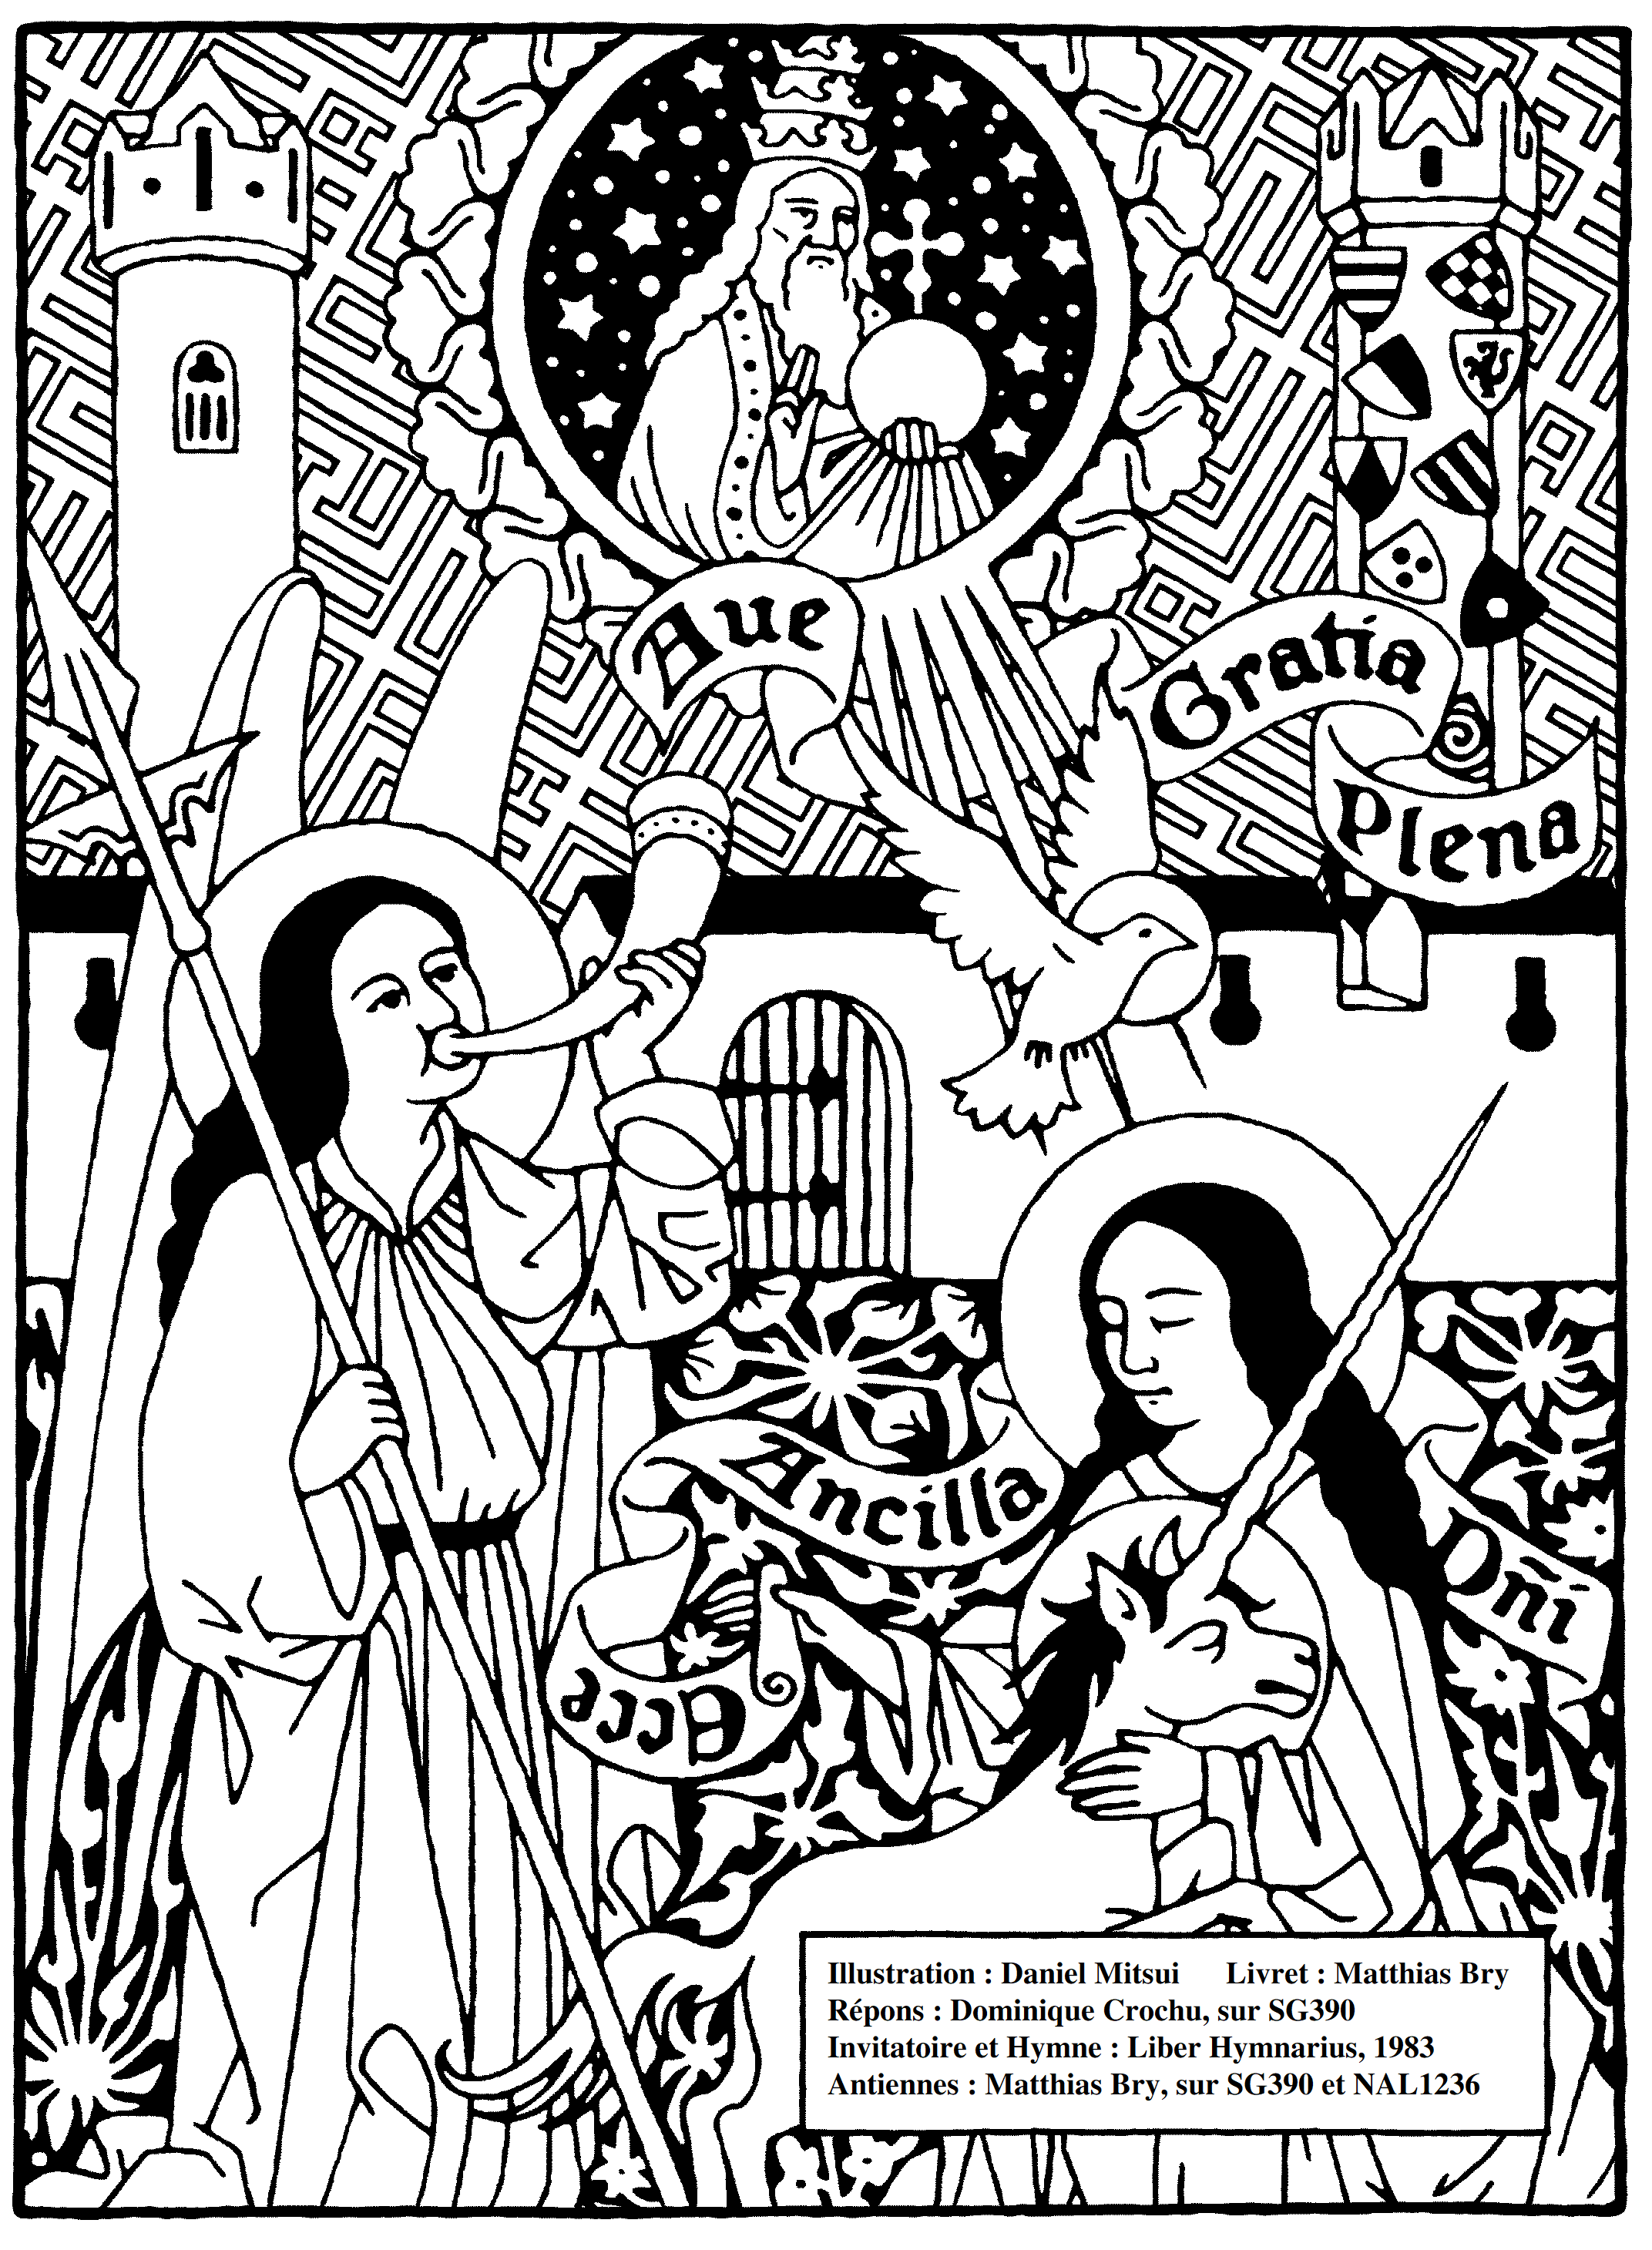
\includegraphics[width=13cm]{4ecouv.png}
\end{adjustwidth}
\end{document} 
